\documentclass[crop,convert={density=300,outext=.png}]{standalone}
\RequirePackage{luatex85}

\usepackage{tikz}
\usetikzlibrary{mindmap,positioning}

\tikzstyle{note} = [text width =5cm, align = left, font=\small]
\begin{document}

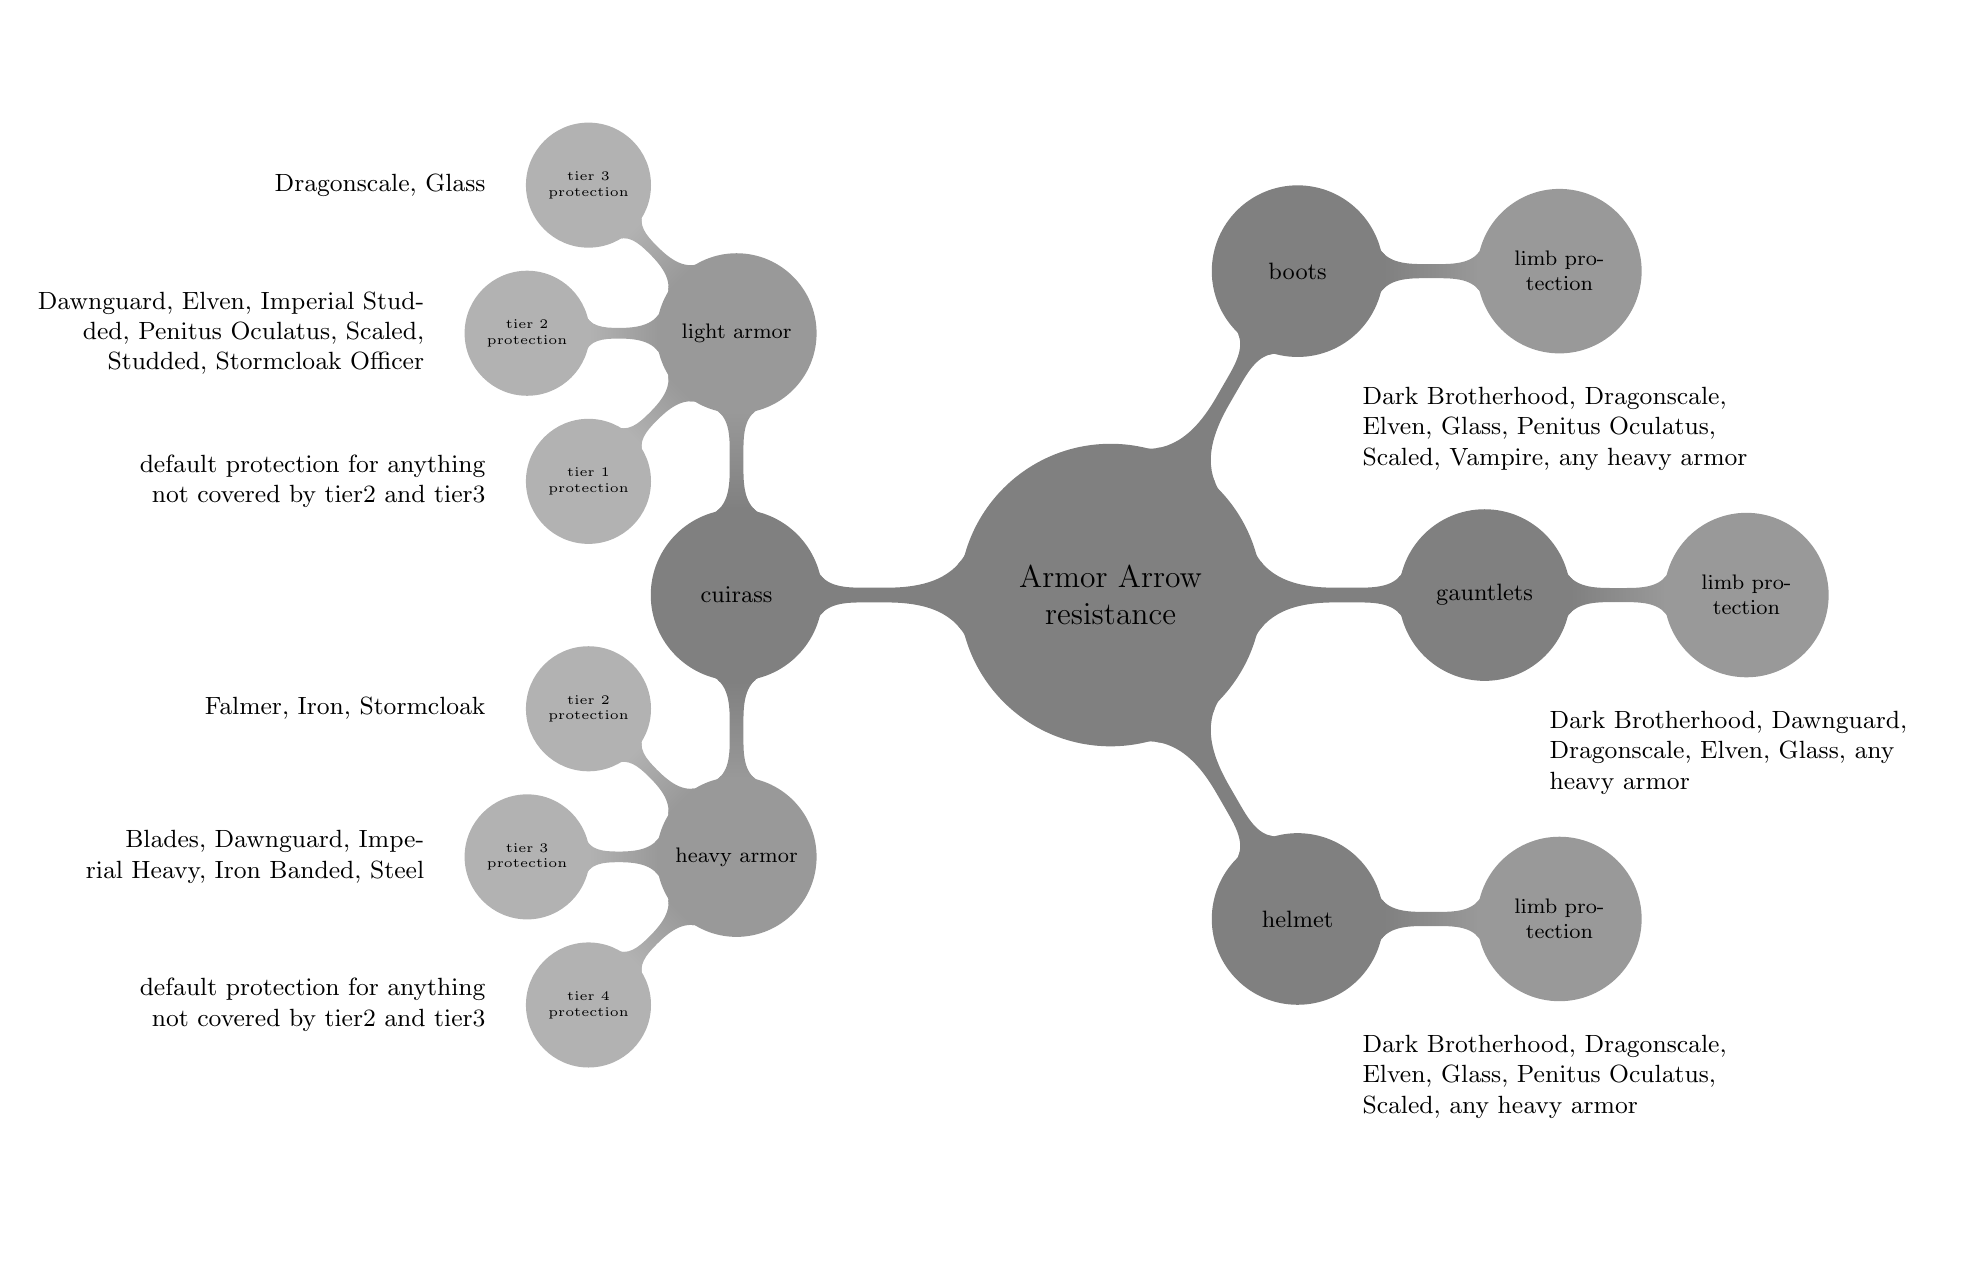
\begin{tikzpicture}[mindmap, scale = 0.95, concept color=black!50]
    \tikzstyle{every concept}+=[scale = 0.95]
    \tikzstyle{root concept}+=[every child/.style={concept color=black!60}]
    \tikzstyle{level 1 concept}+=[every child/.style={concept color=black!50}]
    \tikzstyle{level 2 concept}+=[text width=2cm, level distance = 35mm, every child/.style={concept color=black!40}]
    \tikzstyle{level 3 concept}+=[text width=1.5cm, level distance = 28mm, every child/.style={concept color=black!30}]

    \node [concept, text width=3cm] (root) {Armor Arrow resistance}

    child[grow=180]{
        node [concept] {cuirass}
            child[grow=90] {node [concept] {light armor}
                child[grow=135] {node [concept] (light_t3) {tier 3 protection}}
                child[grow=180] {node [concept] (light_t2) {tier 2 protection}}
                child[grow=225] {node [concept] (light_t1) {tier 1 protection}}
            }
            child[grow=-90] {node [concept] {heavy armor}
                child[grow=135] {node [concept] (heavy_t2) {tier 2 protection}}
                child[grow=180] {node [concept] (heavy_t3) {tier 3 protection}}
                child[grow=225] {node [concept] (heavy_t4) {tier 4 protection}}
            }
    }
    child[grow=60]{
        node [concept] {boots}
            child[grow=0] {node [concept] (boots) {limb protection}
        }
    }
    child[grow=0]{
        node [concept] {gauntlets}
            child[grow=0] {node [concept] (gauntlets) {limb protection}
        }
    }
    child[grow=-60]{
        node [concept] {helmet}
            child[grow=0] {node [concept] (helmet) {limb protection}
        }
    }
        ;
    \node [note, below] at (boots) {
        Dark Brotherhood, Dragonscale, Elven, Glass, Penitus Oculatus, Scaled,
        Vampire, any heavy armor
    };
    \node [note, below] at (helmet) {
        Dark Brotherhood, Dragonscale, Elven, Glass, Penitus Oculatus, Scaled,
        any heavy armor
    };
    \node [note, below] at (gauntlets) {
        Dark Brotherhood, Dawnguard, Dragonscale, Elven, Glass, any heavy armor
    };
    \node [note, align=right, left=0.5cm] at (light_t1.west) {
        default protection for anything not covered by tier2 and tier3
    };
    \node [note, align=right, left=0.5cm] at (light_t2.west) {
        Dawnguard, Elven, Imperial Studded, Penitus Oculatus, Scaled, Studded,
        Stormcloak Officer
    };
    \node [note, align=right, left=0.5cm] at (light_t3.west) {
        Dragonscale, Glass
    };
    \node [note, align=right, left=0.5cm] at (heavy_t2.west) {
        Falmer, Iron, Stormcloak
    };
    \node [note, align=right, left=0.5cm] at (heavy_t3.west) {
        Blades, Dawnguard, Imperial Heavy, Iron Banded, Steel
    };
    \node [note, align=right, left=0.5cm] at (heavy_t4.west) {
    default protection for anything not covered by tier2 and tier3
    };
\end{tikzpicture}

\end{document}